\Large\textbf{}\\
\Large\textbf{Use Case X Creazione nuovo layout} \\
\vspace{0.5cm}
%\begin{figure}[h]
%  \centering
%  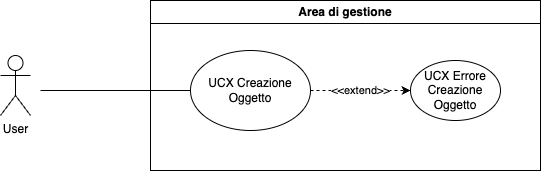
\includegraphics[width=0.8\textwidth]{UseCasesImages/ObjCr.png}
%\end{figure}

\large\textbf{} \\
\textbf{Attori:} User\\
\textbf{Pre-condizione:} Avvio dell'applicazione da parte dell'utente\\
\textbf{Post-condizione: } Creazione del layout magazzino\\
\textbf{Scenario Principale:}  All'utente viene richiesto se caricare un layout esistente o se creare da 0 il layout del magazzino.\\

\vspace{0.5cm}

\Large\textbf{}\\
\Large\textbf{Use Case X Creazione Nuovo magazzino} \\
\vspace{0.5cm}
%\begin{figure}[h]
%  \centering
%  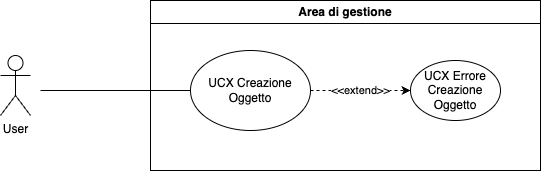
\includegraphics[width=0.8\textwidth]{UseCasesImages/ObjCr.png}
%\end{figure}

\large\textbf{} \\
\textbf{Attori:} User\\
\textbf{Pre-condizione:} E' stato selezionata la modalità: "creazione manuale magazzino" \\
\textbf{Post-condizione: } Creazione del nuovo layout del magazzino\\
\textbf{Scenario Principale:}  L'utente crea un nuovo layout magazzino inserendo le specifiche all'interno di un form prestabilito.\\
\textbf{Estensioni: } UCX Errore Creazione Layout magazzino\\

\vspace{0.5cm}

\textbf{}\\
{\color{red}{\textbf{Domanda:} Il magazzino può avere delle misure arbitrarie? Esistono dei massimi o dei minimi? }} \\
{\color{red}{\textbf{Domanda:} Il magazzino può essere suddiviso in sottoparti? Eventualmente queste sottoparti devono avere delle limitazioni fisiche (muri) o solamente ipotetiche (virtuali)?}}\\

\vspace{0.5cm}

\Large\textbf{}\\
\Large\textbf{Use Case X Importazione layout magazzino} \\
\vspace{0.5cm}
%\begin{figure}[h]
%  \centering
%  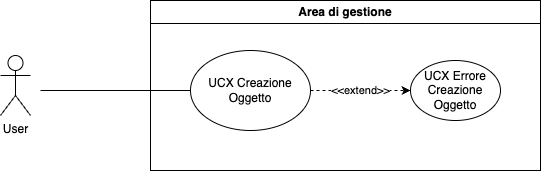
\includegraphics[width=0.8\textwidth]{UseCasesImages/ObjCr.png}
%\end{figure}

\large\textbf{} \\
\textbf{Attori:} User\\
\textbf{Pre-condizione:} E' stato selezionata la modalità: "importazione layout magazzino" \\
\textbf{Post-condizione: } Importazione Layout Magazzino\\
\textbf{Scenario Principale:}  Il magazzino viene correttamente importato da layout esistente.\\
\textbf{Estensioni: } UCX Errore Importazione Layout\\

\vspace{0.5cm}


\Large\textbf{}\\
\Large\textbf{Use Case X Creazione scaffalatura} \\
\vspace{0.5cm}
%\begin{figure}[h]
%  \centering
%  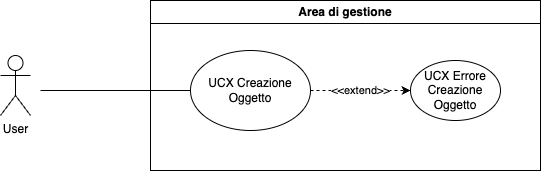
\includegraphics[width=0.8\textwidth]{UseCasesImages/ObjCr.png}
%\end{figure}

\large\textbf{} \\
\textbf{Attori:} User\\
\textbf{Pre-condizione:} Richiesta nuovi inserimento scaffalatura \\
\textbf{Post-condizione: } Creazione corretta della scaffalatura\\
\textbf{Scenario Principale:}  L'utente crea una nuova scaffalatura inserendone le \textit{specifiche caratteristiche}. Se i dati inseriti non rispettano il \textit{criterio prestabilito} viene visualizzato un messaggio di errore.\\
\textbf{Estensioni: } UCX Errore Creazione scaffalatura\\

\vspace{0.5cm}

\textbf{}\\
{\color{red}{\textbf{Domanda:} Una scaffalatura ha delle dimensioni standard o massime? Quanto e se è personalizzabile (sia per le dimensioni effettive della scaffalatura sia per le dimensioni interne degli spazi utili della scaffalatura)? }} \\
{\color{red}{\textbf{Domanda:} Abbiamo delle prescizioni particolari da rispettare? (Come per esempio lo spazio tra una scaffallatura e l'altra; il fatto di poterle "appoggiare una con l'altra") }}\\

\vspace{0.5cm}

\Large\textbf{}\\
\Large\textbf{Use Case X Spostamento scaffalatura} \\
\vspace{0.5cm}
%\begin{figure}[h]
%  \centering
%  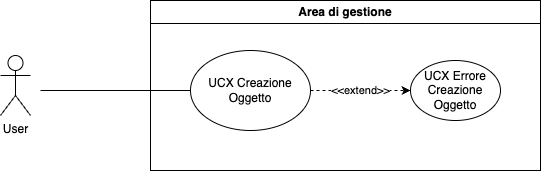
\includegraphics[width=0.8\textwidth]{UseCasesImages/ObjCr.png}
%\end{figure}

\large\textbf{} \\
\textbf{Attori:} User\\
\textbf{Pre-condizione:} Richiesta spostamento scaffalatura \\
\textbf{Post-condizione: } Scaffallatura spostata \\
\textbf{Scenario Principale:}  L'utente selezione la scaffalatura da spostare e il nuovo spazio dove posizionarla.\\
\textbf{Estensioni: } UCX Errore Spostamento Scaffallatura\\

\vspace{0.5cm}

\textbf{}\\
{\color{red}{\textbf{Domanda:} E' uno use case rilevante in termini pratici? E' da implementare? }} \\
{\color{red}{\textbf{Domanda:} Si era pensato di permettere lo spostamento solo a scaffaatura vuota, può essere corretto in termini pratici? }}\\

\vspace{0.5cm}

\Large\textbf{}\\
\Large\textbf{Use Case X Modifica scaffalatura} \\
\vspace{0.5cm}
%\begin{figure}[h]
%  \centering
%  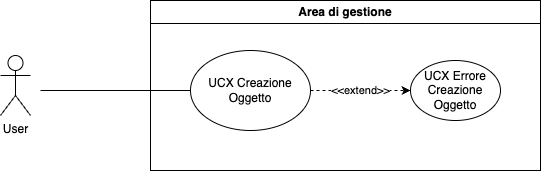
\includegraphics[width=0.8\textwidth]{UseCasesImages/ObjCr.png}
%\end{figure}

\large\textbf{} \\
\textbf{Attori:} User\\
\textbf{Pre-condizione:} Scaffallatura correttamente presente \\
\textbf{Post-condizione: } Corretta modifica scaffalatura\\
\textbf{Scenario Principale:}  L'utente modifica la scaffalatura esistente. \\
\textbf{Estensioni: } UCX Errore modifica scaffalatura\\

\vspace{0.5cm}

\textbf{}\\
{\color{red}{\textbf{Domanda:} Anche in questo caso è possibile modificare solamente la struttura "esterna" della scaffaatura oppure anche gli "spazi interni"? Abbiamo qualche vincolo particolare da rispettare? }} \\

\vspace{0.5cm}